% questions.tex —— 2010 年·普通高等学校招生考试·天津卷·理科 · 题目内容片段（无答案）
% 由 tools/generate_projects.py 依来源总账自 2010/2010_数学真题_天津理_试题.md 生成，勿手改（改源 MD 后重跑）


状态：needs-review；依固定候选 PDF 两页（印刷页 635–636）逐题核验，六幅图已矢量重绘。原页未印分值，不补。

\gkpart{一、选择题}

\begin{question}
\gkti{1}$i$ 是虚数单位，复数 $\dfrac{-1+3i}{1+2i}=$（　）

（A）$1+i$

（B）$5+5i$

（C）$-5-5i$

（D）$-1-i$

\end{question}
\begin{question}
\gkti{2}函数 $f(x)=2^x+3x$ 的零点所在的一个区间是（　）

（A）$(-2,-1)$

（B）$(-1,0)$

（C）$(0,1)$

（D）$(1,2)$

\end{question}
\begin{question}
\gkti{3}命题“若 $f(x)$ 是奇函数，则 $f(-x)$ 是奇函数”的否命题是（　）

（A）若 $f(x)$ 是偶函数，则 $f(-x)$ 是偶函数

（B）若 $f(x)$ 不是奇函数，则 $f(-x)$ 不是奇函数

（C）若 $f(-x)$ 是奇函数，则 $f(x)$ 是奇函数

（D）若 $f(-x)$ 不是奇函数，则 $f(x)$ 不是奇函数

\Needspace{0.4\textheight}
\end{question}
\begingroup
\renewenvironment{question}{\Needspace{0.5\textheight}}{}
\begin{question}
\gkti{4}阅读下面的程序框图，若输出 $s$ 的值为 $-7$，则判断框内可填写（　）
\nopagebreak[4]
\begin{center}% 2010 年天津卷理科第 4 题：程序框图，输出 s = −7 时判断框内的条件。
% 来源 PDF：普通高考/2010/2010天津理.pdf，SHA-256 340aba76699a12f330637f9c682abbc893e03e0e91788287934c0a7e0a3cace9。
% 原页：第 1 页（A3 六栏）第 1 栏中部，书页码 635。
% 重绘依据：开始 → i=1 → s=2 → 判断；是（左）→ s=s−i → i=i+2 → 回到判断前的竖线；
%   否（下）→ 输出 s → 结束。原页判断框内为空。
\begin{tikzpicture}[semithick, >=Stealth,
  every node/.style={inner sep=2pt, font=\small}, node distance=5mm]
  \node (start) [draw, rounded corners=4pt, minimum width=2cm, minimum height=0.55cm] {开始};
  \node (i1) [draw, minimum width=1.6cm, minimum height=0.55cm, below=of start] {$i=1$};
  \node (s2) [draw, minimum width=1.6cm, minimum height=0.55cm, below=of i1] {$s=2$};
  \node (cond) [draw, diamond, aspect=2.2, minimum width=3cm,
    minimum height=1.1cm, below=16mm of s2] {};
  \node (out) [draw, trapezium, trapezium left angle=72, trapezium right angle=108,
    minimum width=2.4cm, minimum height=0.55cm, below=9mm of cond] {输出 $s$};
  \node (end) [draw, rounded corners=4pt, minimum width=2cm, minimum height=0.55cm,
    below=of out] {结束};
  \node (ss) [draw, minimum width=2.6cm, minimum height=0.55cm,
    left=13mm of cond] {$s=s-i$};
  \node (ii) [draw, minimum width=2.6cm, minimum height=0.55cm,
    above=6mm of ss] {$i=i+2$};

  \draw[->] (start) -- (i1);
  \draw[->] (i1) -- (s2);
  \draw[->] (s2) -- (cond);
  \draw[->] (cond) -- node[right] {否} (out);
  \draw[->] (out) -- (end);
  \draw[->] (cond.west) -- node[above, pos=0.72] {是} (ss.east);
  \draw[->] (ss.north) -- (ii.south);
  \draw (ii.north) -- ++(0,0.35) -| ($(s2.south)!0.5!(cond.north)$);
\end{tikzpicture}
\end{center}
\nopagebreak[4]
（A）$i<3?$

（B）$i<4?$

（C）$i<5?$

（D）$i<6?$

\end{question}
\endgroup
\begin{question}
\gkti{5}已知双曲线 $\dfrac{x^2}{a^2}-\dfrac{y^2}{b^2}=1$（$a>0$，$b>0$）的一条渐近线方程是 $y=\sqrt3x$，它的一个焦点在抛物线 $y^2=24x$ 的准线上，则双曲线的方程为（　）

（A）$\frac{x^2}{36}-\frac{y^2}{108}=1$

（B）$\frac{x^2}9-\frac{y^2}{27}=1$

（C）$\frac{x^2}{108}-\frac{y^2}{36}=1$

（D）$\frac{x^2}{27}-\frac{y^2}9=1$

\end{question}
\begin{question}
\gkti{6}已知 $\{a_n\}$ 是首项为 $1$ 的等比数列，$S_n$ 是 $\{a_n\}$ 的前 $n$ 项和，且 $9S_3=S_6$。

则数列 $\left\{\dfrac1{a_n}\right\}$ 的前 $5$ 项和为（　）

（A）$\frac{15}8$ 或 $5$

（B）$\frac{31}{16}$ 或 $5$

（C）$\frac{31}{16}$

（D）$\frac{15}8$

\end{question}
\begin{question}
\gkti{7}在 $\triangle ABC$ 中，内角 $A$，$B$，$C$ 的对边分别是 $a$，$b$，$c$，若 $a^2-b^2=\sqrt3bc$，$\sin C=2\sqrt3\sin B$，则 $A=$（　）

（A）$30^\circ$

（B）$60^\circ$

（C）$120^\circ$

（D）$150^\circ$

\end{question}
\begingroup
\renewenvironment{question}{\Needspace{0.5\textheight}}{}
\begin{question}
\gkti{8}设函数 $f(x)=\begin{cases}\log_2x,&x>0,\\ \log_{\frac12}(-x),&x<0,\end{cases}$ 若 $f(a)>f(-a)$，则实数 $a$ 的取值范围是（　）

（A）$(-1,0)\cup(0,1)$

（B）$(-\infty,-1)\cup(1,+\infty)$

（C）$(-1,0)\cup(1,+\infty)$

（D）$(-\infty,-1)\cup(0,1)$

\end{question}
\endgroup
\begin{question}
\gkti{9}设集合 $A=\{x\mid|x-a|<1,x\in\mathbf R\}$，$B=\{x\mid|x-b|>2,x\in\mathbf R\}$。若 $A\subseteq B$，则实数 $a$，$b$ 必满足（　）

（A）$|a+b|\leqslant3$

（B）$|a+b|\geqslant3$

（C）$|a-b|\leqslant3$

（D）$|a-b|\geqslant3$

\Needspace{0.4\textheight}
\end{question}
\begingroup
\renewenvironment{question}{\Needspace{0.5\textheight}}{}
\begin{question}
\gkti{10}如图，用四种不同颜色给图中的 $A$，$B$，$C$，$D$，$E$，$F$ 六个点涂色，要求每个点涂一种颜色，且图中每条线段的两个端点涂不同颜色，则不同的涂色方法有（　）
\nopagebreak[4]
\begin{center}% 2010 年天津卷理科第 10 题：矩形 ABCD 与两个内点 E、F 的涂色图。
% 来源 PDF：普通高考/2010/2010天津理.pdf，SHA-256 340aba76699a12f330637f9c682abbc893e03e0e91788287934c0a7e0a3cace9。
% 原页：第 1 页（A3 六栏）第 2 栏中部，书页码 635。
% 重绘依据：矩形 ABCD（A 左上、D 右上、B 左下、C 右下），E 在上部与 A、D 相连，
%   F 在下部与 B、C 相连，E 与 F 相连；无矩形的对角线。
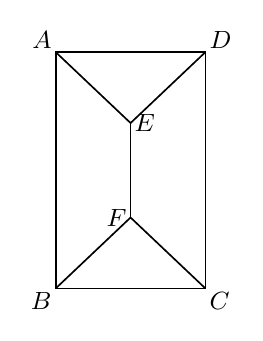
\begin{tikzpicture}[semithick, every node/.style={inner sep=1.2pt, font=\small}]
  \coordinate (A) at (0,3);
  \coordinate (D) at (1.9,3);
  \coordinate (B) at (0,0);
  \coordinate (C) at (1.9,0);
  \coordinate (E) at (0.95,2.1);
  \coordinate (F) at (0.95,0.9);
  \draw (A) -- (D) -- (C) -- (B) -- cycle;
  \draw (A) -- (E) -- (D);
  \draw (B) -- (F) -- (C);
  \draw (E) -- (F);
  \node[above left] at (A) {$A$};
  \node[above right] at (D) {$D$};
  \node[below left] at (B) {$B$};
  \node[below right] at (C) {$C$};
  \node[right] at (E) {$E$};
  \node[left] at (F) {$F$};
\end{tikzpicture}
\end{center}
\nopagebreak[4]
（A）$288$ 种

（B）$264$ 种

（C）$240$ 种

（D）$168$ 种

\end{question}
\endgroup
\gkpart{二、填空题}

\begin{question}
\gkti{11}甲、乙两人在 $10$ 天中每天加工零件的个数用茎叶图表示如图，中间一列的数字表示零件个数的十位数，两边的数字表示零件个数的个位数，则这 $10$ 天甲、乙两人日加工零件的平均数分别为$\underline{\qquad}$和$\underline{\qquad}$。

\begin{center}
\begin{tabular}{ccc}
\toprule
甲 & 十位 & 乙 \\
\midrule
$9\quad8$ & $1$ & $9\quad7\quad1$ \\
$0\quad1\quad3\quad2\quad0$ & $2$ & $1\quad4\quad2\quad4$ \\
$1\quad1\quad5$ & $3$ & $0\quad2\quad0$ \\
\bottomrule
\end{tabular}
\end{center}

\Needspace{0.4\textheight}
\end{question}
\begingroup
\renewenvironment{question}{\Needspace{0.5\textheight}}{}
\begin{question}
\gkti{12}一个几何体的三视图如图所示，则这个几何体的体积为$\underline{\qquad}$。
\nopagebreak[4]
\begin{center}% 2010 年天津卷理科第 12 题：正视图、侧视图与俯视图。
% 来源 PDF：普通高考/2010/2010天津理.pdf，SHA-256 340aba76699a12f330637f9c682abbc893e03e0e91788287934c0a7e0a3cace9。
% 原页：第 1 页（A3 六栏）第 2 栏下部，书页码 635。
% 重绘依据：正视图、侧视图均为宽 1、高 2 的矩形，上方接底宽 2、高 1 的三角形；
%   俯视图为边长 2 的正方形，内含边长 1 的虚线正方形（棱柱顶面），正方形对角线为实线。
\begin{tikzpicture}[semithick, every node/.style={inner sep=1.2pt, font=\small}]
  % 正视图
  \draw (0,4) rectangle (1,6);
  \draw (-0.5,6) -- (0.5,7) -- (1.5,6);
  \draw (-0.5,6) -- (1.5,6);
  \node[below] at (0.5,3.25) {正视图};
  \draw[<->] (-0.9,4) -- (-0.9,6) node[midway,left] {$2$};
  \draw[<->] (-0.9,6) -- (-0.9,7) node[midway,left] {$1$};
  \draw[<->] (0,3.78) -- (1,3.78) node[midway,below] {$1$};
  % 侧视图
  \draw (3,4) rectangle (4,6);
  \draw (2.5,6) -- (3.5,7) -- (4.5,6);
  \draw (2.5,6) -- (4.5,6);
  \node[below] at (3.5,3.25) {侧视图};
  \draw[<->] (2.6,4) -- (2.6,6) node[midway,left] {$2$};
  \draw[<->] (2.6,6) -- (2.6,7) node[midway,left] {$1$};
  \draw[<->] (3,3.78) -- (4,3.78) node[midway,below] {$1$};
  % 俯视图
  \draw (0.5,0) rectangle (2.5,2);
  \draw[dashed] (1,0.5) rectangle (2,1.5);
  \draw (0.5,0) -- (2.5,2);
  \draw (0.5,2) -- (2.5,0);
  \draw[<->] (0.5,-0.38) -- (2.5,-0.38) node[midway,below] {$2$};
  \draw[<->] (0.1,0) -- (0.1,2) node[midway,left] {$2$};
  \node[below] at (1.5,-0.9) {俯视图};
\end{tikzpicture}
\end{center}
\nopagebreak[4]
\end{question}
\endgroup
\begin{question}
\gkti{13}已知圆 $C$ 的圆心是直线 $\begin{cases}x=t,\\ y=1+t,\end{cases}$（$t$ 为参数）与 $x$ 轴的交点，且圆 $C$ 与直线 $x+y+3=0$ 相切，则圆 $C$ 的方程为$\underline{\qquad}$。

\Needspace{0.4\textheight}
\end{question}
\begingroup
\renewenvironment{question}{\Needspace{0.5\textheight}}{}
\begin{question}
\gkti{14}如图，四边形 $ABCD$ 是圆 $O$ 的内接四边形，延长 $AB$ 和 $DC$ 相交于点 $P$，若 $\dfrac{PB}{PA}=\dfrac12$，$\dfrac{PC}{PD}=\dfrac13$，则 $\dfrac{BC}{AD}$ 的值为$\underline{\qquad}$。
\nopagebreak[4]
\begin{center}% 2010 年天津卷理科第 14 题：圆内接四边形 ABCD 与两割线交点 P。
% 来源 PDF：普通高考/2010/2010天津理.pdf，SHA-256 340aba76699a12f330637f9c682abbc893e03e0e91788287934c0a7e0a3cace9。
% 原页：第 1 页（A3 六栏）第 3 栏上部，书页码 635。
% 重绘依据：A、B、C、D 依次在圆上；P 为 AB 与 DC 延长线的交点，
%   连线 A—B—P 与 D—C—P 为割线，另画弦 AD 与弦 BC。
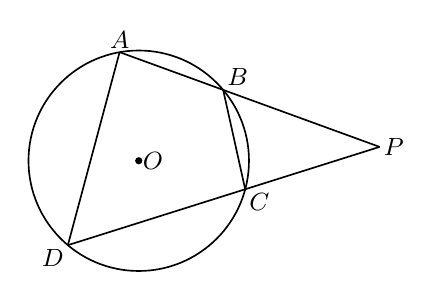
\begin{tikzpicture}[semithick, every node/.style={inner sep=1.2pt, font=\small}]
  \coordinate (O) at (0,0);
  \coordinate (A) at (-0.243,1.379);
  \coordinate (B) at (1.072,0.900);
  \coordinate (C) at (1.352,-0.362);
  \coordinate (D) at (-0.900,-1.072);
  \coordinate (P) at (3.059,0.176);
  \draw (0,0) circle (1.4);
  \fill (O) circle (1.3pt);
  \draw (A) -- (P);
  \draw (D) -- (P);
  \draw (A) -- (D);
  \draw (B) -- (C);
  \node[above] at (A) {$A$};
  \node[above right] at (B) {$B$};
  \node[below right] at (C) {$C$};
  \node[below left] at (D) {$D$};
  \node[right] at (P) {$P$};
  \node[right] at (O) {$O$};
\end{tikzpicture}
\end{center}
\nopagebreak[4]
\Needspace{0.4\textheight}
\end{question}
\endgroup
\begingroup
\renewenvironment{question}{\Needspace{0.5\textheight}}{}
\begin{question}
\gkti{15}如图，在 $\triangle ABC$ 中，$AD\perp AB$，$\overrightarrow{BC}=\sqrt3\overrightarrow{BD}$，$|\overrightarrow{AD}|=1$，则 $\overrightarrow{AC}\cdot\overrightarrow{AD}=$ $\underline{\qquad}$。
\nopagebreak[4]
\begin{center}% 2010 年天津卷理科第 15 题：三角形 ABC 与点 D（D 在 BC 上，AD⊥AB）。
% 来源 PDF：普通高考/2010/2010天津理.pdf，SHA-256 340aba76699a12f330637f9c682abbc893e03e0e91788287934c0a7e0a3cace9。
% 原页：第 1 页（A3 六栏）第 3 栏中部，书页码 635。
% 重绘依据：B、D、C 共线，A 在 BC 上方，AD⊥AB；D 为 BC 内一点。
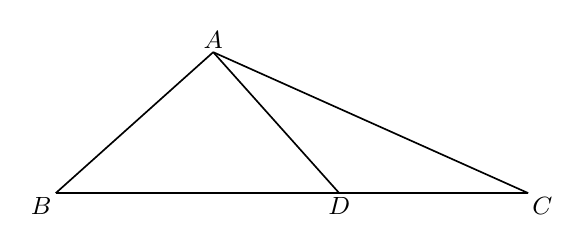
\begin{tikzpicture}[semithick, every node/.style={inner sep=1.2pt, font=\small}]
  \coordinate (B) at (0,0);
  \coordinate (C) at (6,0);
  \coordinate (D) at (3.6,0);
  \coordinate (A) at (2,1.79);
  \draw (B) -- (C);
  \draw (A) -- (B);
  \draw (A) -- (C);
  \draw (A) -- (D);
  \node[above] at (A) {$A$};
  \node[below left] at (B) {$B$};
  \node[below right] at (C) {$C$};
  \node[below] at (D) {$D$};
\end{tikzpicture}
\end{center}
\nopagebreak[4]
\end{question}
\endgroup
\begin{question}
\gkti{16}设函数 $f(x)=x^2-1$，对任意 $x\in\left[\dfrac32,+\infty\right)$，$f\left(\dfrac xm\right)-4m^2f(x)\leqslant f(x-1)+4f(m)$ 恒成立，则实数 $m$ 的取值范围是$\underline{\qquad}$。

\end{question}
\gkpart{三、解答题}

\begin{question}
\gkti{17}已知函数 $f(x)=2\sqrt3\sin x\cos x+2\cos^2x-1$（$x\in\mathbf R$）。

（1）求函数 $f(x)$ 的最小正周期及在区间 $\left[0,\dfrac\pi2\right]$ 上的最大值和最小值；

（2）若 $f(x_0)=\dfrac65$，$x_0\in\left[\dfrac\pi4,\dfrac\pi2\right]$，求 $\cos2x_0$ 的值。

\end{question}
\begin{question}
\gkti{18}某射手每次射击击中目标的概率是 $\dfrac23$，且各次射击的结果互不影响。

（1）假设这名射手射击 $5$ 次，求恰有 $2$ 次击中目标的概率；

（2）假设这名射手射击 $5$ 次，求有 $3$ 次连续击中目标、另外 $2$ 次未击中目标的概率；

（3）假设这名射手射击 $3$ 次，每次射击，击中目标得 $1$ 分，未击中目标得 $0$ 分，在 $3$ 次射击中，若有 $2$ 次连续击中，而另外 $1$ 次未击中，则额外加 $1$ 分；若 $3$ 次全击中，则额外加 $3$ 分。记 $\xi$ 为射手射击 $3$ 次后的总的分数，求 $\xi$ 的分布列。

\Needspace{0.4\textheight}
\end{question}
\begingroup
\renewenvironment{question}{\Needspace{0.5\textheight}}{}
\begin{question}
\gkti{19}如图，在长方体 $ABCD-A_1B_1C_1D_1$ 中，$E$、$F$ 分别是棱 $BC$、$CC_1$ 上的点，$CF=AB=2CE$，$AB:AD:AA_1=1:2:4$。

（1）求异面直线 $EF$ 与 $A_1D$ 所成角的余弦值；

（2）证明 $AF\perp$ 平面 $A_1ED$；

（3）求二面角 $A_1-ED-F$ 的正弦值。
\nopagebreak[4]
\begin{center}% 2010 年天津卷理科第 19 题：长方体 ABCD-A1B1C1D1，E、F 分别在 BC、CC1 上。
% 来源 PDF：普通高考/2010/2010天津理.pdf，SHA-256 340aba76699a12f330637f9c682abbc893e03e0e91788287934c0a7e0a3cace9。
% 原页：第 2 页（A3 六栏）第 1 栏下部，书页码 636。
% 重绘依据：AB:AD:AA1=1:2:4，CF=AB=2CE；可见棱实线，被遮挡的 AB、AD、AA1 虚线；
%   另画平面 A1ED 的 A1E、A1D、ED（虚线）与 AF（虚线）、EF（实线）。
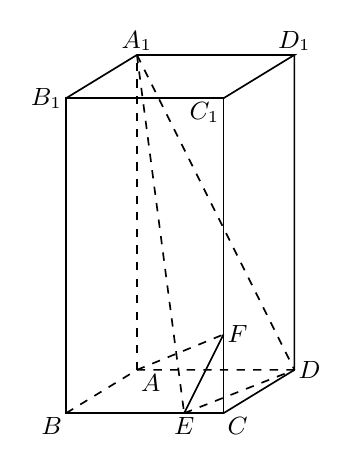
\begin{tikzpicture}[semithick, every node/.style={inner sep=1.2pt, font=\small}]
  \coordinate (B) at (0,0);
  \coordinate (C) at (2,0);
  \coordinate (C1) at (2,4);
  \coordinate (B1) at (0,4);
  \coordinate (A) at (0.9,0.55);
  \coordinate (D) at (2.9,0.55);
  \coordinate (D1) at (2.9,4.55);
  \coordinate (A1) at (0.9,4.55);
  \coordinate (E) at (1.5,0);
  \coordinate (F) at (2,1);
  % 可见棱
  \draw (B) -- (C) -- (C1) -- (B1) -- cycle;
  \draw (B1) -- (A1) -- (D1) -- (C1);
  \draw (D1) -- (D) -- (C);
  % 被遮挡的棱
  \draw[dashed] (B) -- (A) -- (D);
  \draw[dashed] (A) -- (A1);
  % 题设点与辅助线
  \draw (E) -- (F);
  \draw[dashed] (A1) -- (E);
  \draw[dashed] (A1) -- (D);
  \draw[dashed] (E) -- (D);
  \draw[dashed] (A) -- (F);
  \node[above] at (A1) {$A_1$};
  \node[above] at (D1) {$D_1$};
  \node[left] at (B1) {$B_1$};
  \node[below left] at (C1) {$C_1$};
  \node[below left] at (B) {$B$};
  \node[below right] at (C) {$C$};
  \node[right] at (D) {$D$};
  \node[below right] at (A) {$A$};
  \node[below] at (E) {$E$};
  \node[right] at (F) {$F$};
\end{tikzpicture}
\end{center}
\nopagebreak[4]
\end{question}
\endgroup
\begin{question}
\gkti{20}已知椭圆 $\dfrac{x^2}{a^2}+\dfrac{y^2}{b^2}=1$（$a>b>0$）的离心率 $e=\dfrac{\sqrt3}2$，连接椭圆的四个顶点得到的菱形的面积为 $4$。

（1）求椭圆的方程；

（2）设直线 $l$ 与椭圆相交于不同的两点 $A$，$B$。已知点 $A$ 的坐标为 $(-a,0)$，点 $Q(0,y_0)$ 在线段 $AB$ 的垂直平分线上，且 $\overrightarrow{QA}\cdot\overrightarrow{QB}=4$，求 $y_0$ 的值。

\end{question}
\begin{question}
\gkti{21}已知函数 $f(x)=xe^{-x}$（$x\in\mathbf R$）。

（1）求函数 $f(x)$ 的单调区间和极值；

（2）已知函数 $y=g(x)$ 的图象与函数 $y=f(x)$ 的图象关于直线 $x=1$ 对称，证明：当 $x>1$ 时，$f(x)>g(x)$；

（3）如果 $x_1\neq x_2$，且 $f(x_1)=f(x_2)$，证明：$x_1+x_2>2$。

\end{question}
\begin{question}
\gkti{22}在数列 $\{a_n\}$ 中，$a_1=0$，且对任意 $k\in\mathbf N^*$，$a_{2k-1}$，$a_{2k}$，$a_{2k+1}$ 成等差数列，其公差为 $d_k$。

（1）若 $d_k=2k$，证明 $a_{2k}$，$a_{2k+1}$，$a_{2k+2}$ 成等比数列（$k\in\mathbf N^*$）；

（2）若对任意 $k\in\mathbf N^*$，$a_{2k}$，$a_{2k+1}$，$a_{2k+2}$ 成等比数列，其公比为 $q_k$。

① 设 $q_1\neq1$，证明 $\left\{\dfrac1{q_k-1}\right\}$ 是等差数列；

② 若 $a_2=2$，证明 $\dfrac32<2n-\sum\limits_{k=2}^n\dfrac{k^2}{a_k}\leqslant2$（$n\geqslant2$）。

\end{question}